\RequirePackage[l2tabu,orthodox]{nag}

% TODO: decide if one-sided/two-sided
%\documentclass[headsepline,footsepline,footinclude=false,fontsize=11pt,paper=a4,listof=totoc,bibliography=totoc,BCOR=12mm,DIV=12]{scrbook} % two-sided
\documentclass[headsepline,footsepline,footinclude=false,oneside,fontsize=11pt,paper=a4,listof=totoc,bibliography=totoc]{scrbook} % one-sided

% TODO: change citation style in settings
\bibliography{bibliography/literature}{}

\setkomafont{disposition}{\normalfont\bfseries} % use serif font for headings
\linespread{1.05} % adjust line spread for mathpazo font

% Settings for glossaries TODO: remove the following block if glossary not needed
\renewcommand{\glsnamefont}[1]{\normalfont\bfseries #1} % use serif font for glossary entry titles
\makeglossaries{}

% Settings for pgfplots
\pgfplotsset{compat=1.9} % TODO: adjust to your installed version
\pgfplotsset{
  % For available color names, see http://www.latextemplates.com/svgnames-colors
  cycle list={CornflowerBlue\\Dandelion\\ForestGreen\\BrickRed\\},
}

% Settings for lstlistings
\lstset{%
  basicstyle=\ttfamily,
  columns=fullflexible,
  autogobble,
  keywordstyle=\bfseries\color{MediumBlue},
  stringstyle=\color{DarkGreen}
  }


% TODO: change thesis information
\newcommand*{\getUniversity}{Technische Universität München}
\newcommand*{\getFaculty}{Department of Informatics}
\newcommand*{\getTitle}{Design and Prototypical Implementation of a High-Level Synchronization Component for Dynamic Updates of Task Run Queues in L4 Fiasco.OC/Genode}
\newcommand*{\getTitleGer}{Entwurf und Prototypische Implementierung einer High-Level Synchronisationskomponente fuer dynamische Updates von Task-Warteschlangen in L4 Fiasco.OC/Genode}
\newcommand*{\getAuthor}{Gurusiddesha Chandrasekhara}
\newcommand*{\getDoctype}{Master's Thesis in Informatics}
\newcommand*{\getSupervisor}{Prof. Dr. Uwe Baumgarten}
\newcommand*{\getAdvisor}{Daniel Krefft,M.Sc.; Sebastian Eckl,M.Sc.}
\newcommand*{\getSubmissionDate}{November 15, 2016}
\newcommand*{\getSubmissionLocation}{Munich}

\begin{document}

% Set page numbering to avoid "destination with the same identifier has been already used" warning for cover page.
% (see https://en.wikibooks.org/wiki/LaTeX/Hyperlinks#Problems_with_Links_and_Pages).
\pagenumbering{alph}
\begin{titlepage}
  % HACK for two-sided documents: ignore binding correction for cover page.
  % Adapted from Markus Kohm's KOMA-Script titlepage=firstiscover handling.
  % See http://mirrors.ctan.org/macros/latex/contrib/koma-script/scrkernel-title.dtx,
  % \maketitle macro.
  \oddsidemargin=\evensidemargin\relax
  \textwidth=\dimexpr\paperwidth-2\evensidemargin-2in\relax
  \hsize=\textwidth\relax

  \centering

  \vspace{40mm}
  
\includegraphics[width=40mm]{logos/tum}

  \vspace{5mm}
  {\huge\MakeUppercase{\getFaculty{}}}\\

  \vspace{5mm}
  {\large\MakeUppercase{\getUniversity{}}}\\

  \vspace{20mm}
  {\Large \getDoctype{}}

  \vspace{15mm}
  {\huge\bfseries \getTitle{}}

  \vspace{15mm}
  {\LARGE \getAuthor{}}

  \vspace{20mm}
  
\includegraphics[width=20mm]{logos/faculty}
\end{titlepage}

%\afterpage{\blankpage}

\frontmatter{}
\begin{titlepage}
  \centering

  \IfFileExists{logos/tum.pdf}{%
    \includegraphics[height=20mm]{logos/TUMLogo.pdf}
  }{%
    \vspace*{10mm}
  }

  \vspace{5mm}
  {\huge\MakeUppercase{\getFaculty{}}}\\

  \vspace{5mm}
  {\large\MakeUppercase{\getUniversity{}}}\\

  \vspace{10mm}
  {\Large \getDoctype{}}

  \vspace{10mm}
  {\LARGE\bfseries \getTitle{}}

  \vspace{10mm}
  {\LARGE\bfseries \getTitleGer{}}

  \vspace{10mm}
  \begin{tabular}{l l}
    Author: & \getAuthor{} \\
    Supervisor: & \getSupervisor{} \\
    Advisor: & \getAdvisor{} \\
    Submission Date: & \getSubmissionDate{} \\
  \end{tabular}

  \IfFileExists{logos/faculty.pdf}{%
    \vfill{}
    
\includegraphics[height=20mm]{logos/faculty.pdf}
  }{}
\end{titlepage}
%\afterpage{\blankpage}

%\frontmatter{}
%\afterpage{\blankpage}
\thispagestyle{empty}
\vspace*{0.8\textheight}
\noindent
I confirm that this \MakeLowercase{\getDoctype{}} is my own work and I have documented all sources and material used.

\vspace{15mm}
\noindent
\getSubmissionLocation{}, \getSubmissionDate{} \hspace{5cm} \getAuthor{}

\cleardoublepage{}

%\afterpage{\blankpage}

\addcontentsline{toc}{chapter}{Acknowledgments}
\thispagestyle{empty}

\vspace*{20mm}

\begin{center}
{\usekomafont{section} Acknowledgments}
\end{center}

\vspace{10mm}

%TODO: Acknowledgments

%Writing this master's thesis would not have been possible without the help of these people. 
%First, I would like to thank my advisors Daniel Krefft and Sebastian Ekcl, who immediately accepted my request to do masters thesis and guided me to chose the projects. Special thanks to Daniel Krefft for his brilliant advices which he has given me every time we had a discussion.
%
%Thanks to Prof.Baumgarten for allowing me to do my research and for providing all the facilities at the chair. 
%
%Thanks to Paul Nieleck, who is finished his master thesis at the department for excellent collaboration and sharing his knowledge on the project. 
%
%Thanks to Alexander Reisner who is working at the department, for sharing his timely invaluable experience on the project. 
%
%%Thanks to Madhura Kumaraswamy for her help during my thesis. 
%
%Thank you to my family for providing me the freedom and support that required me to come to Germany for doing my masters. 


\cleardoublepage{}


\chapter{\abstractname}

%TODO: Abstract

%Motivation/Problem statement Aims and objectives

This thesis introduces a method for updating the task ready queues in the Genode Operating System Framework and the L4/Fiasco.OC microkernel. The presented method will be used in Organic Computing paradigm's Observer-Controller architecture. The Observer monitors the system and gathers the data and passes it to the Controller, which processes the data and takes a decision to schedule the tasks. This requires a method in place to provide the synchronized access to ready queue and update the tasks.

%What does the thesis do?
%The limitations in accessing the kernel ready queue from a high-level component led to the development of a split module. Accordingly,
The implementation of the ready queue update mechanism consists of a high-level Genode component and a low-level kernel module. The Genode component communicates with the Controller via a shared dataspace and receives the tasks to be updated and then passes them to the kernel module. The kernel module identifies the corresponding kernel threads and updates them to the ready queue. Various synchronization methods are presented in this thesis with special importance to lock-free algorithms. RCU and STM synchronization methods are suggested for synchronizing the kernel ready queue access. 

%Findings and conclusions
Tests of the task-ready queue update mechanism showed that the threads can be updated successfully to the ready queue and executed. On the other hand, complete ready queue swapping leaves the system in an unstable state. The high-level component is able to communicate successfully with the Controller via Genode's shared dataspace. The proposed design and implementation can be successfully used in the Observer-Controller architecture and it serves as a good starting point for the KIA4SM project's goal of having the ready queue update mechanism as a fully high-level component.

%vision of providing a homogeneous execution environment for heterogeneous hardware systems involves in using universally applicable ECUs and having flexible task scheduling on ECUs. This requires having a intelligent system in place to take decisions, which is solved by Organic-Computing paradigm's Observer-Controller architecture, which has an Observer that monitors the system and gathers the data and pass it to the Controller, which processes the data and takes a decision to schedule the tasks. This requires a method in place to provide the synchronized access to ready queue and update the tasks.

\microtypesetup{protrusion=false}
\tableofcontents{}
\afterpage{\blankpage}
\microtypesetup{protrusion=true}

\newpage
\addcontentsline{toc}{chapter}{Acronyms}
\chapter*{Acronyms}

\begin{acronym}[EDF]
	\acro{ECU}{Electronic Control Unit}
	\acro{IPC}{Inter Process Communication}
	\acro{ITS}{Intelligent Transportation System}
	\acro{KIA4SM}{Cooperative Integration Architecture for Future Smart Mobility Solutions}
	\acro{EDF}{Earliest Deadline First}
	\acro{FP}{Fixed Priority}
	\acro{IPC}{Inter-Process Communication}
	\acro{SMP}{Symmetric Multi Processing}
	\acro{RPC}{Remote Procedure Calls}
	\acro{OC}{Organic Computing}
	\acro{OC}{Object Capability System}
	\acro{PD}{Protection Domain}
	\acro{API}{Application Programming Interface}
	\acro{RCU}{Read Copy Update}
	\acro{STM}{Software Transactional Memory}
	\acro{CPU}{Central Processing Unit}
	\acro{OS}{Operating System}
	\acro{L4Re}{L4 Runtime Environment}
	\acro{QEMU}{Quick Emulator}
	\acro{RAM}{Random Access Memory}
	\acro{RM} {Region Manager}
	\acro{RQ}{Ready Queue}
	\acro{UTCB} {User-level Thread Control Block}
	\acro{GNU}{GNU's Not Unix}
	\acro{GCC}{GNU Compiler Collection}
	\acro{GMBH}{full name}
	\acro{GPL}{full name}
\end{acronym}

\mainmatter{}

% !TeX root = ../main.tex
% Add the above to each chapter to make compiling the PDF easier in some editors.

\chapter{Introduction}\label{chapter:introduction}

The implemented low-level synchronization component in this master thesis is part of the KIA4SM project of the chair of operating systems. The work aims to implement a method for dynamic update of tasks ready queues in L4 Fiasco.OC/Genode while providing a synchronized access to them.


\section{Overview of KIA4SM project}

KIA4SM (stands for Cooperative Integration Architecture for Future Smart Mobility Solutions) is a research project at the department of operating systems \cite{kia4sm}. Traditionally Cooperative Intelligent Transport Systems(C-ITS) have been built on heterogeneous systems. The KIA4SM project aims to provide an architecture of having homogeneous software platform for heterogeneous hardware systems. The project focuses on developing systems for the interaction and coordination between
computer-assisted vehicles, be it partially or fully autonomously functioning actors and also aims to improve on the ad-hoc networking between vehicles

The final vision of the project is illustrate in figure \ref{kia4sm}. The goals of the project are,

\begin{figure}[h]
  \centering
  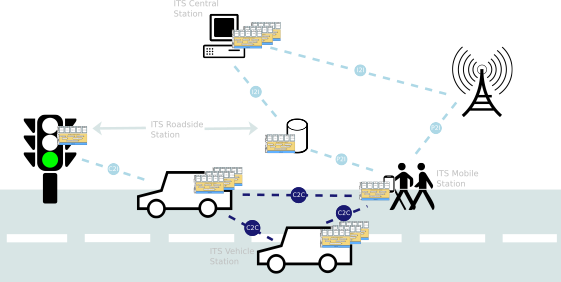
\includegraphics[scale = 1]{figures/kia4sm_vision.png}
  \caption{KIA4SM vision - homogeneous platform for heterogeneous devices \cite{kia4sm}} \label{kia4sm}
\end{figure}

\begin{itemize}
\item A common platform as foundation for device independent (vehicles, mobile devices, traffic and
transport architecture) provision and execution of software-based functionality
\item Mechanisms that allow for online dynamic reconfiguration, based on
\begin{itemize}
\item en-/disabling and relocation/migration of
software-based functionality
\item adaptive (data-centric) routing policy
\item flexible scheduling of tasks per ECU
\end{itemize}
\end{itemize}

In order to achieve the goals of the project a number of different methods have been applied. This has led to the application of Organic computing paradigm.
Organic Computing (OC) has the vision to address the
challenges of complex distributed systems by making them more
life-like (organic), i.e. endowing them with abilities such as self-
organization, self-configuration, self-repair, or adaptation.
%Refer: paper: Organic Computing – Addressing Complexity by Controlled Self-organization 
In order to realize this, universally applicable Electronic Control Units (ECU) and a common run-time environment are used which provides Hardware/Software Plug-and-Play properties.

\section{Motivation}

There are number of micro controllers used for different calculations in a modern vehicle, KIA4SM project aims to replace them with use of more power-full and standardized hardware, universally applicable ECUs. 

OC approach proposes a Observer-Controller architecture similar to MAPE architecture(monitor, analyze, plan, execute) . An observer collects the data from the all the ECUs and computes and generates indicators where a controller takes a decision based on the indicator and generates an action.

One such action of the controller is to decide what tasks should be executed at what time in order to meet the aforementioned requirements of the safety critical systems. It is essential to be able to add threads and modify the execution order during operation time.
A flexible thread handling is also required for example in case 
a ECU is malfunctioning. In this case it would be possible to swap the threads from the 
malfunctioning one to working ones. So it is important to generate new ready-queues 
based on the information we are receiving from the other ECUs in the grid, and then 
exchange them with the actual ready-queue the scheduler uses. 

The controller decides and produces a run/ready queue (RQ). There needs to be a method which allows to safely update the scheduler ready queue of the system. The work in this thesis concentrates on the scheduler ready queue update mechanism.

\begin{figure}[h][architecture]
  \centering
  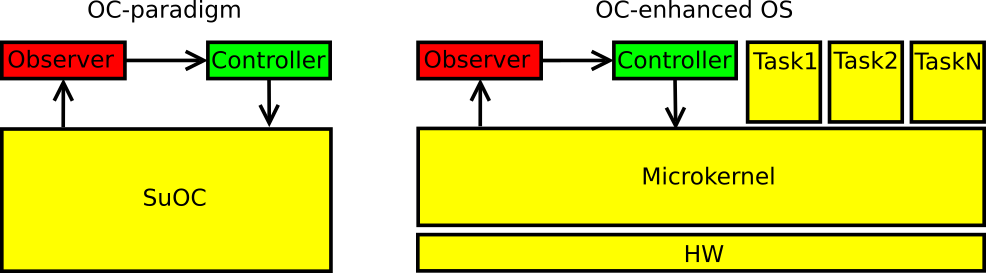
\includegraphics[scale = 0.5]{figures/microkernel_architecture.png}
  \caption{Organic Computing: Applying the Observer/Controller pattern to existing microkernel architecture \cite{kia4sm}}\label{architeture}
\end{figure}

\section{Thesis structure}
The thesis is structured in a way that the reader understands the importance of the work carried out here and also the surrounding concepts before delving in to the specifics (inverted triangle). 

The second chapter summarizes the related work on the state of the art algorithms for synchronization and different types of schedulers in use and at the end of the section an evaluation of the synchronization methods is provided in order to chose the best possible approach for the existing project.

The third chapter explains the Genode and L4 Fiasco.OC details in brief, in order for the user to have an overview of the system. 

The fourth chapter deals with the design considerations along with implementation details.

The fifth chapter is dedicated to explains testing method and the results obtained.
And the final chapter concludes the thesis with the limitations and future work to be done. 
\afterpage{\blankpage}
\chapter{Related Work}
This chapter explains the previous work and concepts which led to the development of synchronization component to the KIA4SM project and it explains the synchronization algorithms available and makes a comparative study of these algorithms. 
The comparative study is based on the research work of papers which are referred here. An attempt is made to pick the best choice algorithm for the work. 

\section{Synchronization of L4 fiasco tasks}

The thesis is largely based on the work of Robert H{\"a}cker, who in his bachelor thesis \textit{ "Design of an OC-based Method for efficient Synchronization of L4 Fiasco.OC Mircrokernel Tasks"} \cite{haecker}, explains the design of a scheduler best suited scheduler for KIA4SM project and also gives comparison study of the different schedulers and synchronization methods suited for updating the task ready queue. 

He suggests Modified-Maximum-Urgency-First(MMUF) algorithm as the best choice for KIA4SM project due to the importance of safety and security in embedded systems. After comparing the synchronization algorithms the sequential lock technique has been chosen for the better control it gives. He has suggested to verify the practical implication of Read-Copy Update(RCU). At the end, he proposes a design for the existing system including aforementioned  scheduler(MMUF) and sequential locks. 

This work is an extension of H{\"a}cker's findings. However, the focus of the thesis it to develop a good synchronization method, the implementation of the scheduler is not carried out.

Some of the ideas and code knowledge is taken from the Valentin Hauner's bachelor's thesis \textit{"Extension of the Fiasco.OC microkernel with context-sensitive scheduling abilities for safety-critical applications in embedded systems"} \cite{hauner}. In this thesis he added EDF scheduling strategy. Though his thesis concentrated on using it in Genode and L4RE environment, it helped in understanding the Fiasco.OC's scheduler.

\section{Synchronization Methods} \label{rq:sync}
To do the justification to many synchronization methods are studied and are explained in this section. The synchronization categories are divided based on the methods they apply. 
The figure %TODO insert the picture 
shows the different types of synchronization methods along with examples. 

\subsection{Lock Based Algorithms}
Lock based algorithms are a simple way of enforcing the limits on access to shared resource, where there are multiple threads of execution. A lock enforces a mutual exclusion concurrency control. The area where the read or write is happening to a shared resource is called critical section. The thread has to acquire a lock before entering the critical section, only one thread can acquire this lock and whenever it leaves the critical section the thread should release the lock, so that the other threads can enter critical section.

There are many different types of lock based synchronization methods exists.

\begin{labeling}{lock}
\item[Mutex] Mutex is a synchronization primitive stands for mutual exclusion, which prevents the simultaneous access to shared resource. The thread which wants to execute in critical section has to acquire the mutex and after it leaves it has to give the mutex. 

\item[Semaphore] It's a variable used to control the common resource access between multiple processes/threads. A typical semaphore is initialized with an initial value which is equaled to the number of resources are available and the value is decremented whenever a process takes the resource. If the value of the semaphore is 0 then all the resources are empty and the thread/process has to wait. This works in the opposite way for the event management, where initial value is 0 and semaphore is increased every time an event occurs and decremented when the corresponding event is processed. A binary semaphore has only two values(0 and 1) and works similar to mutex.   

\item[Spin-lock] It's a type of lock, where the thread wants to access the critical section waits in a loop (spin) while trying to acquire the lock. The thread remains active on the CPU while no useful work is being done. Spin locks have very good advantage if the threads are blocked for shorter periods of time.
\end{labeling} 

The lock based synchronization primitives are simple, easy to implement. However, there exist a lot of disadvantages. If the programmer is not careful, deadlocks can occur and are difficult to debug. One interesting problem might arrive is priority inversion, which is defined for two threads i and j as, if J is in critical section, assign J to highest priority and when it exits critical section assign its original priority. The problem with priority inversion is, a higher thread has to wait for the lower priority thread, which is not desirable for real time systems. 

Another problem includes thread starvation, where a thread doesn't get CPU time due to long waits, which is again problem for safety critical systems, since threads should reach their deadline.
 
\subsection{Lock-Free Algorithms}

Lock Free algorithms refer to a synchronization methods where the access to critical section for all the threads is guaranteed without using the locks. Two major algorithms are discussed in the category of lock free algorithms.

\textbf{Read-Copy Update:}
Read-Copy Update (RCU) guarantees concurrent read and write operations to the same data.  It's a synchronization mechanism that was added to the Linux kernel during the 2.5 development effort that is optimized for read-mostly situations. RCU achieves scalability improvements by allowing reads to occur concurrently with updates \cite{whatisrcu}. Compared to conventional locking primitives, which ensures mutual exclusion among concurrent threads regardless of read/write operation, RCU supports concurrency between single updater and multiple readers. This is achieved in RCU by keeping multiple versions of variables and ensuring that they are not freed up until all the pre-existing readers have finished using the old copies of the variable. RCU uses three main mechanisms to achieve lock-free synchronization method which are,

\begin{labeling}{rcumethods}
\item[\textbf{Publish-Subscribe Mechanism (for insertion)}:]
Publish subscribe mechanism is a way of enforcing the compiler to execute the instructions in correct order. If a pointer is getting updated, an rcu call(rcu\_assign\_pointer())  is used to change the pointer. This can be thought of as publishing the data. This requires the readers also should wait for the update to happen to read the correct data, the dereferencing of the pointer is done by using an rcu call(rcu\_dereference()), which is further guarded by rcu read lock.

\item[\textbf{Wait For Pre-Existing RCU Readers to Complete (for deletion)}:]
The figure \ref{fig:rcu_grace} shows this mechanism in picture, where RCU's way of waiting for existing reader threads to finish. RCU introduces a grace period, where it waits on read-side critical section. The simple way to find out when the reader threads have finished the critical section is to check for the context switch of the CPU. 

\begin{figure}[h]
\centering
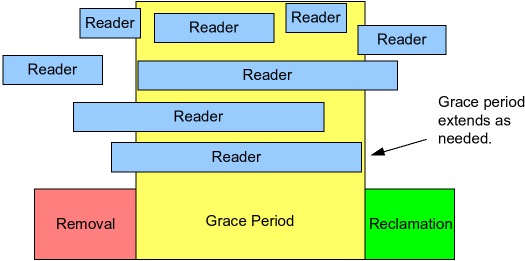
\includegraphics[width=0.7\linewidth]{figures/rcu_grace}
\caption{RCU showing the usage of grace period \cite{whatisrcu}}
\label{fig:rcu_grace}
\end{figure}

\item[\textbf{Maintain Multiple Versions of Recently Updated Objects (for readers)}]:
RCU maintains the multiple versions of the data in between removal and reclamation phases. The figure \ref{fig:rcu} shows how RCU maintains the multiple versions of data. In the linked list, B has to be removed. The first phase is changing the link from A to C, but the link from B to C still exists(removal phase). This way, if any readers were at B, they can reach C and any new readers will see only A to C. When the grace period ends, memory for B is freed(reclamation phase).

\begin{figure}[h]
\centering
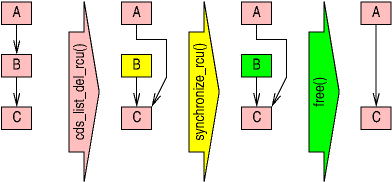
\includegraphics[width=0.7\linewidth]{figures/rcu}
\caption{Ready copy update mechanism, showing deferred destruction \cite{whatisrcu}}
\label{fig:rcu}
\end{figure}
\end{labeling}

Since the introduction of RCU, there has been lot improvements made. The research from McKenney \emph{et al.} shows that RCU can provide order-of-magnitude speedups for read-mostly data structures \cite{whatisrcu}. RCU is optimal when less than 10\% of accesses are updates over wide range of CPUs. Sarma \emph{et al.} work on making the RCU suitable for real-time systems improves on carefully RCU callbacks. They suggest three methods such as,  providing per-CPU kernel daemons to process RCU callbacks, directly invoking the RCU callback and throttling the RCU callbacks so that the limited number are invoked at a given time \cite{sarma2004making}.

\textbf{Software Transactional Memory:}
Software Transactional Memory (STM) is a concurrency control mechanism works in a similar way to database transactions by providing atomic and isolated execution for regions of code. The instructions to access shared memory are executed in a transaction, so the other threads will not see any changes when a thread is executing instructions in a transaction. At the end either the transaction is committed(if no other threads have modified the data) or aborted and the transaction is restarted. 

STM requires language extensions and compiler takes care of data versioning and conflict detection mechanisms and makes sure that the global state of the program is consistent. From GCC 4.7, STM support has been added, which makes it ideal to use in this project. The code listing shows the example transaction execution in GCC.


\begin{lstlisting}[caption={STM example code in GCC},label=sysdeploycode, style=customcpp]
void testfunc(int *x, int *y){
_transaction_atomic{
*x += *y;
}
}
\end{lstlisting}

Other nonblocking data structures which are being researched in embedded systems and other operating system groups are, 

\begin{labeling}{waitfree}
\item[\textbf{Wait-free algorithms:}] A Wait-free implementation of a concurrent data object guarantees that a thread executes in a finite number of steps, regardless of execution times of other threads  \cite{herlihy1991wait}. For example, when a higher priority thread A detects that a lower priority thread B is in critical section that A wants to enter, A lends B its priority to let B finish the execution. When B has finished, A executes in its own critical section.


\item [\textbf{Lock-free synchronization:}] It works completely without locks, this is done by using an atomic update operation like Compare-and-Swap(CAS). \textit{Critical code sections are designed such that they prepare their results out of line and then try to commit them to the pool of shared data using an atomic memory update instruction} \cite{hohmuth2001pragmatic}. It works in two steps, \textit{compare} step detects the conflict between two threads that are updating the memory location. In case of failure the whole operation is restarted. This gives deadlock free code but requires that primitives for atomic memory update operations are available.
\end{labeling}



\section{Evaluation of Synchronization techniques}

\begin{center}
\begin{tabular}{|l|l|l|p{3cm}|}
\hline 
\textbf{Criteria} & \textbf{Mutex} & \textbf{RCU} & \textbf{STM} \\ \hline

Implementation & + & - - & ++ \\ \hline

Read-speed & - - & ++ & + \\ \hline

Write-speed & - - & + & + \\ \hline

Deadlocks & - - & ++ & + \\ \hline

Overhead & + & + & - - \\ \hline

Security/Consistency & ++ & - & + \\ \hline
\end{tabular}
\captionof{table}{ Evaluation of synchronization techniques}\label{tab:lock}
\end{center}

The evaluation of these methods are according to the study of the above mentioned papers and the work of Heaker's analysis. Lock based methods and STM are easy to implement since the language constructs provide the mechanism. STM is better than locks, because with using many locks code can become unreadable while STM code has better readability \cite{pankratius2014software}. RCU is hard to implement, since the developer has to take care of providing all the read side locks, grace period handling, list operations etc.

RCU is better to use when there are multiple readers, so the read speed is very good while write-speed is still better than locks, which perform the worst in read and write speed since only one thread can access and other threads need to wait. STM's read and write is good, but only drawback it might have to read again, if the data changes in the middle of the transaction.

There is no deadlock problem in RCU, while the deadlocks are common in locks. STM also suffers from data races. RCU and locks have less overhead compared to STM. STM has to keep the logs of the transaction and has to take care to roll-back if something goes wrong. The data is consistent at all times while using locks but this is not same for RCU and STM. RCU has multiple versions of the data and STM has the logs and keeps the old data.

The recent research in STM is increasing, Ferad \emph{et al.} research suggests that implementing STM from scratch is better than trying to convert the programs from locks to STM \cite{zyulkyarov2009atomic}. The research from Victor \emph{et al.} \cite{pankratius2014software} showed that  TM is very good tool but needs C++ language refinements and better debugging support and large transactions can hurt the performance.

RCU seems a better choice for using in updating the ready queues but also it adds considerable code, given the fact that it's a embedded system. The practical approach of implementing a lock based and a lock free algorithm makes   a better case to find out the preferred method.

%\section{System Requirements} \label{foundations_cons}
%Since the system in use is a safety-critical real time system, there are certain factors to be considered in proposing a solution to the system.
%
%\begin{enumerate}
%
%\item Since the system is a safety-critical real time system, the safety becomes major criteria. The system should be in a predictable state always and is able to gracefully handle any error state.
%
%\item Any solution that is proposed should be efficient, since the used system is a embedded system. Since the system contains the less memory and processing power, the code should be simple and efficient.
%
%\item The utilization of the CPU should be intelligent to ensure that the all threads reach their deadline, since the computed value of no use once the deadline has passed. This requires a effective scheduling strategy to be used. 
%
%\end{enumerate}
\chapter{ Foundations} \label{foundations}
Genode operating system framework and L4/Fiasco is used as the preferred kernel in this project. Since the kernel itself acts a type-I Hypervisor which allows for partitioning of different software components via separated container, making them work on user mode level \cite{kia4sm}.

To understand the design and implementation of this project, the reader has to be aware of few important concepts in both Genode operating system and L4 Fiasco.OC kernel. Many concepts here are the relevant parts explained from the Genode book \cite{genodebook} according to author's understanding, but the reader can always refer to the book for detailed explanation.

\section{Genode Operating System Framework} \label{foundations_genode}
Genode operating system  framework is a tool kit for building secure, special purpose operating systems. Genode is maintained by German company Genode Labs GMBH, which  offers both commercial licenses  and open-source license under GPLv2. The operating system can be used as an embedded operating system or a fully sophisticated general purpose operating system. 

Genode operating system uses a recursive tree structure, where each node in the tree represents a component. Each node is owned by its parent and it controls every aspect of its child like resource control, execution environment etc. The root of the tree is a minimalistic microkernel, which is responsible for providing protection domain, threads of execution and communication mechanism between the protection domains. The rest of the operating system's features such as, device drivers, network stacks, file systems, virtual machines are the nodes of the operating systems. Each component gets a share of the physical resources available. The components can grant the resources to its children. If the components wants additional resources it can request its parent, where the parent can grant or deny it.

This makes Genode operating system to have less trusted computing base(TCB) and gives better security features. If a parent thinks that a child is compromised, it can destroy the child while keeping the rest of the system safe. Genode operating system has been developed to strike a balance between various aspects of operating systems. For example, OS has to provide an assurance that threads get fair share of execution time while accommodating rich and dynamic workloads and similarly for security features and user friendliness.

Genode supports both x86 and ARM CPU architectures and it can be used with most members of L4 family(NOVA, Fiasco.OC, OKL4 v2.1, L4ka::Pistachio, Codezero, L4/Fiasco) of micro kernels. And on Fiasco.OC it supports paravirtualization, a virtualization technique that provides an interface to virtual machines that are similar to their underlying hardware. This method can be effectively used to solve safety related issues of the mixed-criticality system such as the one presented in the KIA4SM project. This makes a very good choice of operating system to use for KIA4SM project.

\subsection{Source Tree Structure}
At the root of the directory there are 3 folders, \texttt{doc/} which contains the documentation in and the release notes of all versions. \texttt{tool/} folder for build systems and tools used in the system and finally \texttt{repos/} which contains the source-code repositories. 

Inside the \texttt{repos/} folder \texttt{base/} repository contains the basic framework related code and \texttt{base-<platform>/} folders contain the platform specific code, where <platform> refers to foc, which contains related code for Fiasco.OC etc.

\subsection{Capabilities, RPC Objects, Protection Domain}\label{Foundations:cap}
Genode consists of many components and each component lives in a \texttt{protection domain}, which provides an isolated execution environment. The resource is abstracted to an \texttt{RPC object} and a token which gives access to this RPC object is called \texttt{capability}.

When RPC object is created, Genode creates a so called \texttt{object-identity} which represents the RPC object in kernel space. The kernel maintains a capability space, which holds reference for the object identities. This capability space is explained in detail in \ref{founcations:overfiasco}
The capabilities can be passed to different components, this operation of transferring capability from one protection domain to another is called  \texttt{delegation}

\subsection{Client-Server Relationship}
Capabilities are used to call methods of RPC objects which are from different protection domains. The component that uses the RPC object is called client and the owner of the RPC object plays the role of the server. The server should at-least have one thread called \texttt{entrypoint}, which gets activated whenever when the client calls the method.

Clients generally have to trust the server since they are granted from the parent through session invocation. Servers do not trust their clients and cancel the service anytime if it detects a security threat.

 
\subsection{Component Creation}
Genode component is made up of five basic parts, 

\begin{labeling}{component}
\item[RAM session] Allocates memory for program's BSS and heap
\item[ROM session] Contains executable binary
\item[CPU session] creates initial thread of the component
\item[RM session] manages the component's address space 
\item[PD session] represents the protection domain
\end{labeling}

As mentioned earlier each Genode component is created out of a parent and the parent is responsible for granting these sessions to child. 

\subsection{Inter-component Communication}\label{Foundations:icc}
Genode provides three principle mechanisms for inter-component communication namely synchronous remote procedure calls (RPC), asynchronous notifications, and
shared memory. Synchronous RPC is the prominently used communication mechanism in the Genode world, since this not only able to transfer the information but has the ability to delegate the capabilities and has the authority throughout the system. 
RPC mechanism is similar to a way the function calls work, where control transfer between caller and callee happens. Synchronous RPC mechanism uses kernel's IPC to transfer messages between client and server. The asynchronous notification is helpful when the caller doesn't want to wait for the control to come back. The Synchronous RPC mechanism can be used in this work but there might be a bulk transfer of data between Controller and Synch component. So the idea of Shared memory concept came as a replacement and is very well suited.

The steps taken in allocating and using shared dataspace are,
\begin{enumerate}
\item The first step is allocating the memory, server does this by interacting with core's RAM service to allocate new RAM dataspace. This space is owned by server

\item The server attaches dataspace to its own RM session. This makes the dataspace contents available in it's virtual address space.

\item Server delegates the authority to client whenever a request for the dataspace.

\item The client can attach the obtained dataspace from the server to its own RM session to access the contents
\end{enumerate}

All of these methods are rarely used in isolation and most of the communication methods are used in combination of these methods. In this particular work RPC and shared memory are used in combination.

\subsection{Interaction with Kernel}
The interaction of user-level threads with the kernel can be seen as a state machine with state transitions. The user-level threads in Genode enter the kernel via a system call, either by device interrupts or by a CPU exception. Once entered, the kernel takes the corresponding action for the event that caused the kernel entry, and the thread leaves the kernel to the user land.

One such kernel interaction is scheduling a thread. Scheduler maintains a list of so called scheduling contexts and each of these refers to a thread. Each time the kernel is entered, the scheduler is updated with the passed duration. When updated, it takes a scheduling decision by making the next to-be-executed thread the head of the list. At kernel exit, the control is passed to the user-level thread that corresponds to the head of the scheduler list.

\subsection{Trace Service}
Genode has a Trace service, which can be used by the user level components for light weight event-tracing. This can be used for obtaining the thread related information for all the threads available in the system. This service is used in the testing of the thread update mechanism which will be explained later in chapter \ref{chap:testing}.

\section{Overview of L4/Fiacso.OC} \label{founcations:overfiasco}
Fiasco.OC is a 3rd generation capability-based microkernel which belongs to L4 family of microkernel. Fiasco provides multi processor support and hardware assisted virtualization and paravirtualization. It is capable of real-time scheduling and is scalable from embedded to HPC systems \cite{foc_feat}. These features made Fiasco.OC has the ideal choice for using in this project. Fiasco.OC can used with L4 Runtime Environment (L4Re), which provides necessary support to develop applications or with an operating system such as Genode.

The OC in Fiasco.OC stands for Object capability system. In this kernel everything is represented as an object and they interact with each other with kernel provided IPC mechanism. Since the system is built around objects, where each object provides a service which other objects can use. The capabilities in Fiasco.OC represents references to the kernel objects and are stored in a per task capability mapping tables which increases the security of the kernel. The figure \ref{fig:foc_cap} \cite{foc_pdf}, shows the per task capability table. Kernel provides a factory for object management.

\begin{figure}[h]
\centering
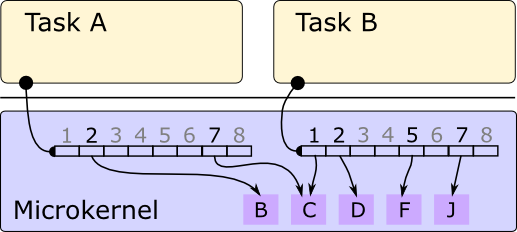
\includegraphics[width=0.7\linewidth]{figures/foc_cap.png}
\caption {Per process capability table in Fiasco.OC \cite{foc_pdf}}
\label{fig:foc_cap}
\end{figure}

The table \ref{tab:foc_kobject} shows the kernel provided objects.
\begin{center}
\begin{tabular}{|l|p{10cm}|}
\hline 
\textbf{ Kernel Object} & \textbf{Description} \\ \hline

Task & Represents a protection domain in which the threads can execute\\ \hline

Thread & Unit of execution in a task
\\ \hline

Factory & Used for creation of kernel objects \\ \hline

IPC Gate &  Kernel provided IPC channel\\ \hline

IRQ & Interrupt request signal object used for asynchronous signaling\\ \hline

ICU & Hardware interrupt request controller \\ \hline

Scheduler &  The scheduler object managing the CPUs \\ \hline
\end{tabular}
\captionof{table}{ The Fiasco.OC kernel objects}\label{tab:foc_kobject}
\end{center}

The kernel has a object space which contains the capabilities to objects. This can be considered as a pool of objects and a look can be done with the given id to find out the object. Fiasco.OC uses so called flex pages which are passed via IPC and are used to identify the kernel objects. A thread object in Fiasco.OC represents a execution unit and belongs to a task which provides a protection domain for the thread to execute. The thread has 3 states in Fiasco.OC, \texttt{ready, running, blocked} states. 

The thread holds a User-level Thread Control Block(UTCB), mainly used for system call parameters and has following contents,
\begin{itemize}
\item MR message registers, contains untyped message data and items

\item BR buffer registers, receive buffers for capabilities

\item TCR thread control registers used for error codes and user values
\end{itemize}

The \texttt{Thread class} implemented in kernel acts as a driver class which controls most of the functionality. The execution of thread has scheduling context and an execution context which are explains in the next section.


\subsection{Scheduler Context}\label{Foundations:sc}
Steinberg - who developed Quality assuring scheduling in the Fiasco Microkernel explains some of the concepts of the Fiasco in his thesis \cite{stein}. Steinberg decouples the execution and scheduling in order to help with the IPC and thread time donation in Fiasco microkernel. In which a new class is introduced called Sched\_Context containing all the scheduling and accounting parameters. And the class that implements execution contexts is called Context

The regular scheduling context becomes part of the TCB and additional scheduling contexts for each thread via SLAB allocator. This separation of execution and scheduling context allows the system to do fast IPC (The sender of an IPC donates its time quantum to receiver, which gets activated and avoids the invocation of the scheduler). During the execution of a thread, kernel switches to the execution context and the scheduling context of the thread to be executed. When a situation arrives where the thread is donating its time and priority to other thread, the kernel has to only switch the execution context of the destination thread and the scheduling context remains the same.

The scheduling context object is implemented in a \texttt{sched\_context} class and the \texttt{Context} class represents the execution context or thread.

The table \ref{tab:sched} shows the scheduling context's attributes and their meaning.
\begin{center}
\begin{tabular}{|l|p{9cm}|}
\hline 
\textbf{Attribute} & \textbf{Description} \\ \hline

Owner & This is a pointer, which points to the owner thread of the scheduling context\\ \hline

ID & A positive number to identify the scheduling context, the regular scheduling context is assigned 0
\\ \hline

Prio & Priority of the scheduling context \\ \hline

Quantum &  The total time quantum associated with the scheduling context\\ \hline

Left & The remaining time of the original time quantum \\ \hline

Prev, Next & Pointers pointing to the next and previous scheduling contexts \\ \hline

Per\_cpu<Ready\_queue> rq &  Processor specific ready queue \\ \hline

Sc\_type & Enum object, the type of the scheduler (Fixed priority or EDF) \\ \hline

Deadline & In case of EDF scheduler, the deadline of a thread \\ \hline
\end{tabular}
\captionof{table}{ The attributes of scheduling context}\label{tab:sched}
\end{center}

\subsection{Ready Queue}\label{Foundations:rq}
The ready queue holds a list of threads which are ready to be executed next. The Fiasco.OC microkernel supports 256 priorities ranging from 0 to 255. In case of fixed priority scheduler, there is a list exists for each of the priority levels. The scheduler works in round robin fashion, where it picks the head of the highest priority thread to execute, it runs until a certain time quantum and choses the next thread in the list. In case there are no threads to be executed in the highest priority list, the scheduler picks the thread from next highest priority list. 
Note to be taken in Fiasco.OC kernel the thread that is on the CPU will not be in the ready queue, once the thread finishes it's allocated CPU time for the run, it is re-queued back to the ready queue list(provided it's time quantum still exists).

In Fiasco.OC \texttt{prio\_next[256]} represents the ready queue list and uses a variable called \texttt{prio\_highest} to determine the highest priority available.  

\subsection{Enqueue and Dequeue Operation}	
Modification of ready queue operation is a critical section. The uniprocessor implementation uses a simple CPU lock to disable the interrupts and SMP processors uses CPU specific ready queue operation. In order to use per CPU ready queue list, the kernel has to ensure the preemption is disabled. Enqueue operation takes a scheduler context object to be enqueued and checks if it's already in the list. This is checked against the corresponding priority list. If the thread is not in the ready queue list, it is enqueued and prio\_highest variable is set accordingly. 

The dequeue operation is similar to enqueue, after disabling the CPU preemption, it deletes if the thread exists in the list. Once the operation is completed the CPU preemption is enabled.

\section{Thread Creation calls in Genode and Fiasco.OC}\label{foundations:thread_creation}

\begin{figure}[h]
\centering
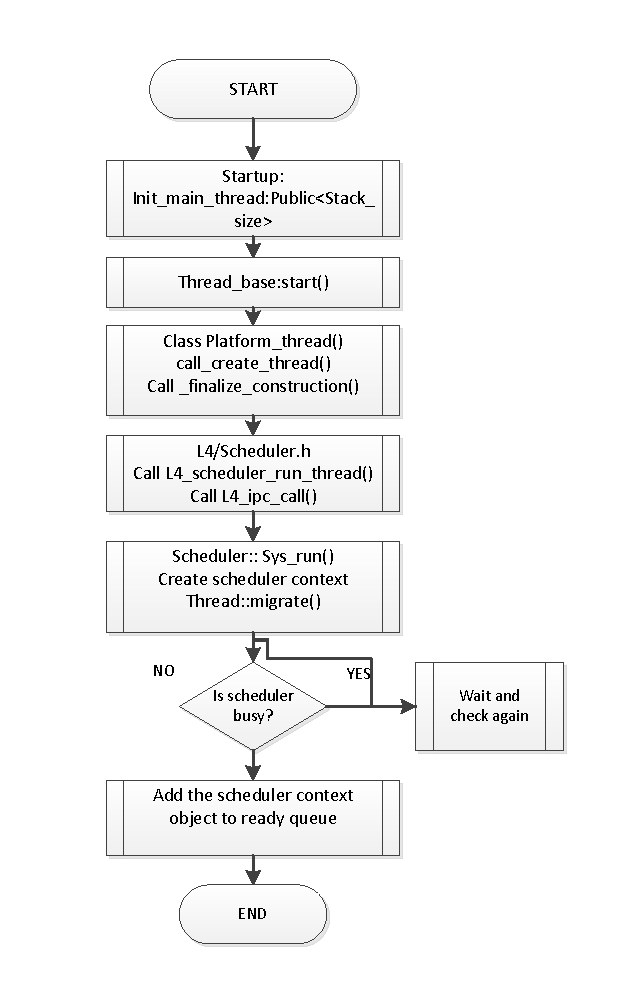
\includegraphics[width=0.7\linewidth]{figures/Thread_creation}
\caption{Thread creation calls in Genode operating system}
\label{fig:Thread_creation}
\end{figure}

Thread creation Genode application is done by creating a class and inhering the Genode \texttt{Thread} class. This class takes stack size as template parameter. The diagram \ref{fig:Thread_creation}
shows the sequence of calls taken from application to all the way down the kernel level.  
The derived class needs to have a constructor and an entry function. The entry function implements the work done by the thread. When the thread objects are created and the start method of the Genode Thread class is called, the entry method starts executing. The code listing \ref{threadcreate} shows the inhering the Thread class to create user threads.

\begin{lstlisting}[caption={Thread creation class},label={threadcreate}, style=customcpp]
class Mythread : public Genode::Thread<2*4096>
{
	public:

		Mythread() : Thread("MyThread") { }

		void entry()
		{
			printf("I'm a thread\n");
			// Some useful work
		}
};
\end{lstlisting}

Once the Genode application creates the thread the sequence of calls take place.

\begin{enumerate}
\item The kernel specific code takes over in the Genode, In case of Fiasco.OC, the call goes to \texttt{base-foc/src/core/Platform\_thread.cc}. Platform\_thread.cc implements the major functionalities to interact with the kernel, such as creating the thread, setting the thread related values, selecting the affinity space and priorities for the thread etc. Further there are two types of platform\_thread constructors available. One for the core threads which takes just the name of the argument and other for user level threads which takes the name and priority of the thread.  The platform thread constructor calls \texttt{\_create\_thread} and \texttt{\_finalize\_construction }.

\item The \_create\_thread calls l4\_factory\_create\_thread API with the L4\_BASE\_FACTORY\_CAP and threads local ID. This call creates L4 thread in kernel. 

\item The \_finalize\_construction calls L4 APis to create IRQ, set the name of a thread in kernel and sets the scheduling parameters (l4\_scheduler\_run\_thread).

\item \texttt{l4\_scheduler\_run\_thread} makes an IPC call to scheduler kernel object, by which kinvoke call of the scheduler object is invoked.

\item The sys\_run call identifies the thread and scheduling parameters associated with it. The scheduler\_context object is created with the defined scheduling strategy(FP or EDF). The thread is then migrated to the corresponding CPU and added to the ready queue.  
\end{enumerate}

\section{Creating a Kernel Object in Fiasco.OC}\label{implement:kernelobject}
In this section creating a new kernel object is explained, that can be utilized to make a dedicated work in the kernel. The following changes are required to create kernel object and compile it. A new class should be created, which inherits \texttt{Icu\_h<object name>} and
\texttt{Irq\_chip\_soft} classes. The class has to declare this as kernel object using a macro (FIASCO\_DECLARE\_KOBJ()) provided from Fiasco.OC and the memory is allocated outside the class by defining the kernel object and sending the class name as a parameter. The class has to have a static object created inside the class and an interrupt request(Irq\_base) object defined in it. In the constructor of the class it is important to register this object to initial kernel objects. 

The class definition and the registering of kernel object can be seen in listing \ref{kobject}. The new object is called \texttt{RQ\_manager}, which should take care of the ready queue handling.

\begin{lstlisting}[caption={Creating new kernel object},label=kobject, style=customcpp]
class RQ_manager : public Icu_h<RQ_manager>, public Irq_chip_soft
{
  FIASCO_DECLARE_KOBJ();
  typedef Icu_h<RQ_manager> Icu;

public:
  enum Operation
  {
	RQ_info = 0,
	Schedule_thread = 1,
  };

  static RQ_manager rq_manager;
private:
  Irq_base *_irq;
};

FIASCO_DEFINE_KOBJ(RQ_manager);

PUBLIC inline
RQ_manager::RQ_manager() : _irq(0)
{
  initial_kobjects.register_obj(this, 8);
}

PUBLIC
L4_msg_tag
RQ_manager::kinvoke(L4_obj_ref ref, L4_fpage::Rights rights, Syscall_frame *f,
                   Utcb const *iutcb, Utcb *outcb)
{
}

enum Protocol{
  Label_rq_manager = -22L,   // Protocol ID for rq manager objects<l4_types.cpp>
}
enum l4_msgtag_protocol{
L4_PROTO_RQ_MANAGER = -22L, //Protocol for messages to a rq_manager object<types.h>
}

static Cap_index const C_rq_manager = Cap_index(8); //kernel-thread-std.cpp
\end{lstlisting}

This class should implement few of the functions from the inherited classes such as \texttt{icu\_bind\_irq} and \texttt{icu\_set\_mode} and a \texttt{kinvoke} call which the Fiasco uses it to do interprocess communication.

This created kernel object needs to be associate with protocol ID. These protocol IDs are used for either
kernel implemented objects and this is assigned in the \texttt{l4\_types.h}, protocol section of the
l4\_msg\_tag and also it needs to be assigned with l4\_msgtag\_protocol. This kernel object is assigned a \texttt{Cap\_index} which it was registered against.
\chapter{Design}\label{design}

This chapter gives a high-level overview of the  design of \texttt{Observer-Controller} architecture used in the KIA4SM project. It also describes the design details of  the \texttt{Synchronization} module and the communication architecture between the \texttt{Synchronization} module and \texttt{Controller} module.

\section{Overview}

\begin{figure}[h]
  \centering
  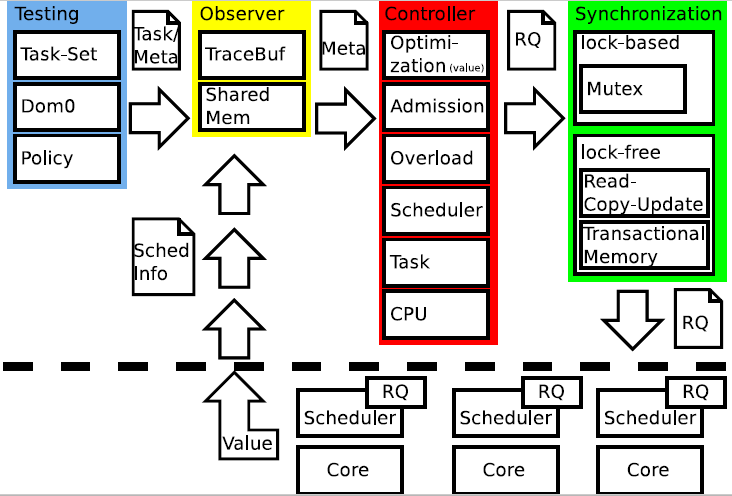
\includegraphics[scale = 0.7]{figures/oc.png}
  \caption{The Observer- Controller architecture}\label{oc}
\end{figure}

The figure \ref{oc} shows the \texttt{Observer-Controller} architecture. Its goal is to have a system that can automatically take the decisions of scheduling tasks/threads by observing the system. There are three main modules involved, namely, \texttt{Observer}, \texttt{Controller} and \texttt{Synchronization}. All these modules are implemented as Genode OS applications (or components).

The \texttt{Observer}'s (also called Monitor/Monitoring agent) job is to collect all the information from the system, analyse it and send it to the \texttt{Controller}. The \texttt{Observer} collects the information by using the \texttt{Trace} facility available in Genode. The data collected from the \texttt{Observer} includes \textit{number of tasks}, \textit{process ID}, \textit{execution time of each task}, \textit{RAM info}, \textit{CPU quota}, etc.

The \texttt{Controller} is responsible for maintaining the system in a safe and optimized state. It analyses the data collected from the \texttt{Observer} and takes a decision for system reconfiguration\cite{kia4sm}. The system reconfiguration involves updating a single thread to the ready queue or generating a new ready queue. It then communicates the system reconfiguration data to the \texttt{Synchronization} module. The \texttt{Controller} also applies load balancing or energy saving techniques to keep the system in an optimized state.

The design of \texttt{Synchronization} component is quite complicated. The initial design consisted of having a high-level component, which can directly access the kernel ready queue and exchange it with the ready queue given by the \texttt{Controller}. This requires synchronized access to the kernel ready queue. However, further research showed that this design required modification due to the following reasons:  

\begin{itemize}
\item Kernel ready queue cannot be directly accessed from a high-level component such as the one proposed, since the kernel protection domain prevents direct access.

\item The \texttt{Controller} cannot create the ready queue that can be directly used by the kernel. This is because the
thread ids represented in Genode OS framework differ from the thread ids in the kernel. Moreover, the ready queue list in the kernel has scheduler context objects in it (explained in \ref{Foundations:rq} and \ref{Foundations:sc}). Hence, a user-level component such as the \texttt{Controller} cannot access scheduler context objects.

\item The list type for ready queue is implemented in a template class called \texttt{Dlist}, which is accessible only from the kernel and needs a re-implementation in the user-level component.

\end{itemize}

\begin{figure}[h]
	\centering
	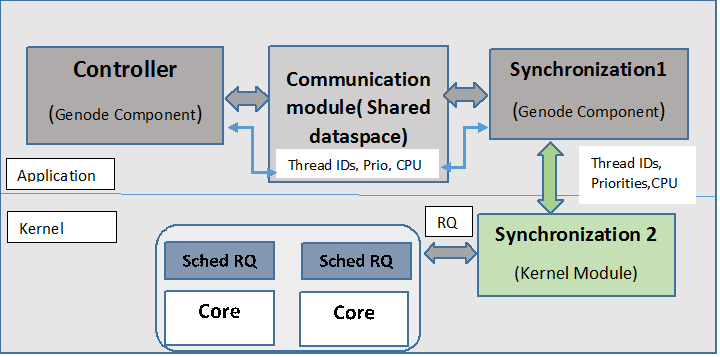
\includegraphics[width=0.7\linewidth]{Abstract_design.png}
	\caption{The synchronization module design with communication and Controller}
	\label{fig:abstractdesign}
\end{figure}


The high-level view of the new design is depicted in figure \ref{fig:abstractdesign}.
The Synchronization module is split into two major parts. The first part is implemented as a high-level Genode component, which is responsible for communicating with the \texttt{Controller} and passing the data to the second part. The \texttt{Controller} and the \texttt{Synchronization} module interaction is that of a producer-consumer relationship. The producer (\texttt{Controller}) produces a thread (or ready queue) and a consumer (\texttt{Synchronization} module) consumes the thread by updating it to the kernel ready queue. This needs a synchronization mechanism to be implemented between these two components (see \ref{rqmodule}).

The second part of the \texttt{Synchronization} module is responsible for taking the thread data from the user-level component and updating the threads to the ready queue. It is implemented in the Genode operating system, with most of the work done in L4/Fiasco.OC microkernel. It has to ensure that the access to the ready queue is synchronized. It should also makes sure that the updated threads execute and the system is in safe state.

Figure \ref{fig:Design_25} shows the data and control flow, and the interfaces between the modules of the new design.

\begin{figure}[h]
\centering
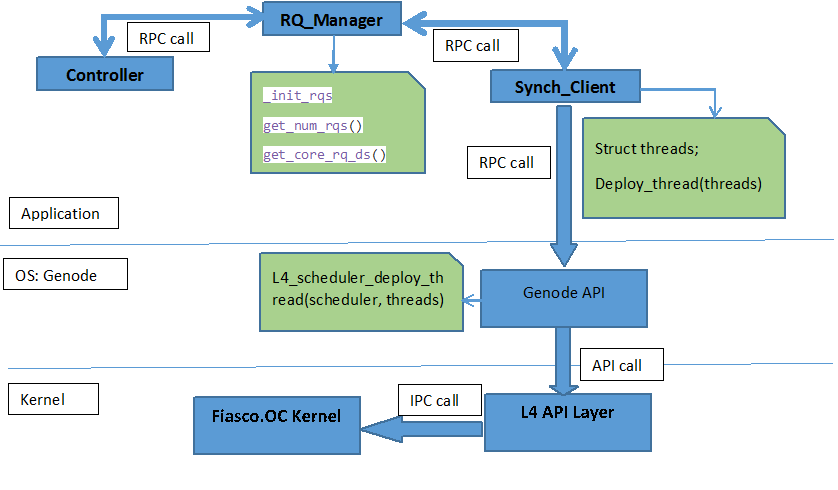
\includegraphics[width=1.0\linewidth]{figures/Design_25.png}
\caption{The data flow between Synch component, Rq manager and Controller}
\label{fig:Design_25}
\end{figure}

The \texttt{Rq\_manager} is a Genode component and is responsible for providing the communication interface between \texttt{Controller} and \texttt{Synchronization}. The main aim is to have a fast communication between the components in order to reduce latency. The best choice for providing a communication interface in Genode is to create a shared dataspace, as explained in section \ref{Foundations:icc}. The \texttt{Rq\_manager} acts as a server in Genode by providing its services to the clients. This is the first component created in the execution sequence, and it provides RPC interface to its clients. This component is only required to provide the initial communication interface and dataspace management. The clients which access the server's services can directly communicate with each other once they obtain the shared dataspace. 

The \texttt{Controller} and the \texttt{Synch\_client} are Genode components and act as clients to the \texttt{Rq\_manager}. The \texttt{Controller} uses the Genode RPC calls to obtain the dataspace capability from \texttt{Rq\_manager}. Once it has the access, it updates the dataspace with thread information. This information consists of the Genode OS framework thread ids, processor id on to which the thread is to be scheduled, and the priorities of the threads. However, the \texttt{Controller} doesn't enforce any policies to the \texttt{Synch\_client}. So, both these components work independently from each other but are synchronized via dataspace.

The \texttt{Synch\_client} also uses the Genode RPC calls to obtain the dataspace capability from \texttt{Rq\_manager}. Once it obtains the access to shared dataspace, it checks for the thread information and transfers the thread ids, priorities and CPU information to the kernel. The communication between Genode and Fiasco.OC kernel is governed by L4 API calls. However, the \texttt{Synch\_client} being a high-level Genode component, cannot make use of L4 API calls by itself. In order to communicate with the kernel, the \texttt{Synch\_client} makes use of Genode OS framework's service. It first creates Genode's RPC object, then using this, it makes a call to the API of Genode's RPC object. The Genode's RPC object makes an API call to the L4 layer. The L4 API communicates the information to Fiasco.OC kernel object by using the IPC service provided by the kernel. The kernel threads are identified by the kernel and updated to the ready queue.

The following sections give detailed design of the individual modules.

\section{Rq\_manager module}\label{rqmodule}
The communication part of the work was collaborated with Paul Nieleck, who worked on the \texttt{Controller} part of the \texttt{Observer-Controller} architecture\cite{paul}. As Nieleck designed and implemented this module, only the details that help to understand the \texttt{Synchronization} component are described below. 

The \texttt{Rq\_manager} has two main functionalities. First, creating a shared dataspace using Genode's APIs and providing a mechanism to access and modify the shared dataspaces to its clients. The \texttt{Rq\_manager} acts as a server in Genode's client-server relationship. It interacts with the Core's RAM service and obtains a RAM dataspace. The Core’s RAM service returns a dataspace capability after allocating memory. Then, the \texttt{Rq\_manager} attaches the dataspace to its RM session and whenever a client requests this dataspace capability, the server delegates it. Once the clients obtain the dataspace capability, they can attach it to their own RM session and access the contents inside the dataspace. Now, both the server and clients have access to shared memory via their respective virtual addresses.

\section{Synch\_client module}
The \texttt{Synch\_client} module is a Genode component that is responsible for updating the threads to the ready queue. It communicates with the \texttt{Controller} using a shared dataspace created by the \texttt{Rq\_manager}. This acts as a client to the \texttt{Rq\_manager} and obtains the dataspace capability from the \texttt{Rq\_manager} via an RPC call. It does so by creating a Connection object provided by the \texttt{Rq\_manager}. This is also responsible for transferring the thread update information to the kernel.

Once the dataspace is accessible, the \texttt{Synch\_clinet} runs in an infinite loop to continuously check the dataspace for any thread that needs to be scheduled. Once it finds such a thread, it updates the thread to the ready queue and then, informs the \texttt{Controller} about the scheduling by updating the shared dataspace. This way, the \texttt{Controller} knows whether the thread scheduling was successful.

The \texttt{Synch\_client} also communicates with the kernel. However, this is done by using the Genode's Trace service. It creates a Connection object provided from the Genode's Trace service to make an RPC call to the Trace object. It makes RPC call with the thread information and waits for the call to return. The return value indicates the success/failure about updating the threads to the kernel ready queue. The \texttt{Synch\_client} then updates this information to the shared dataspace so that the \texttt{Controller} can take a scheduling decision.

\section{Ready queue update Mechanism} \label{design:rqupdate}
 
 Ready queue update mechanism is the process of reading the ready to execute threads and making sure that they are updated in the respective ready queues of the processors. Figure (class diagram, which involves, Synch\_client to scheduler class ) %TODO
shows the high level overview of the involved classes in this process.
A Genode module provides an API, which can be called from the \texttt{Synch\_clinet}. The L4 module provides API calls, which can be called from Genode. The Fiasco.OC kernel module accesses the incoming threads and updates them to the ready queue.

The following subsections give an overview of the modules shown in figure (class diagram)%TODO

\subsection{Genode module}
Genode module is a component which provides an API that can be called from the \texttt{Synch\_client} to communicate with L4/Fiasco.OC kernel. Since L4 calls cannot be made directly from the application, a Genode helper component is necessary to make these calls. The Genode API acts as a wrapper to the L4 calls. It takes the information from the \texttt{Synch\_client} and copies it to the data structure used by the kernel and calls L4 API. The call to L4 is a blocking one. It waits for the L4 call to return and checks for the success or failure. Based on the return value of the L4 API, the Genode module returns 1 (ready queue update successful) or 0 (ready queue update failure) to the \texttt{Synch\_client}.

\subsection{L4 module}

The L4 module represents the L4 API layer, which governs the communication between Genode and Fiasco.OC. It provides an API written in L4sys code, which is called from the Genode module. It is responsible for obtaining the thread ids from Genode and pass them to the Fiasco.OC module using an L4 IPC call. The L4 provides many facilities to the kernel, such as utilities for different platforms, GCC libraries and L4 system calls (L4sys). Once the thread ids are obtained from the Genode API, it extracts and fills them in the kernel's UTCB(used for transferring function call parameters) to make the IPC call.

Additionally, the L4 module is also responsible for converting the thread ids to kernel understandable flex pages (explained in \ref{imp:l4api}). Once the IPC call returns, this module returns the same value to the Genode module. 

\subsection{Fiasco.OC Kernel module}

The Fiasco.OC kernel module is responsible for receiving the threads from the L4 API and safely updating them to the ready queue list of the scheduler. The figure %TODO
shows the involved classes, data and control flow between these classes.

There were two design choices available to receive the incoming threads from L4 API. The first one was to use an existing kernel object (scheduler) and the second was to create a new kernel object (see \ref{implement:kernelobject}). The second method ensures that the legacy code is clean and provides a dedicated object. However, it uses extra memory and adds the complexity of maintaining one more kernel object. So, the idea of using the scheduler object was used in designing this module. 

The scheduler kernel object is used to get the thread data from the L4 API. The obtained thread information is in the form of L4 flex pages. These pages are converted to get the thread ids, which can be used to obtain the scheduler context objects. A list is created similar to the ready queue list using the scheduler context objects. This module then makes a decision about when the ready queue should be updated according to the current state of the system. After the decision, it calls the methods in the ready queue class to update/exchange the list.

The call is then transferred to the Sched\_context\_Fp\_EDF class. The type of the ready queue is selected depending on the type of the scheduler in use. If it is a Fixed priority scheduler, an exchange call is made to the FP ready queue class. 

The FP exchange call receives the new ready queue list and the priority. A call is made to the list data type to switch the ready queue. A boolean value is returned to the scheduler to indicate the success.

Additionally, this module has to provide a synchronized access to the ready queue. The synchronization method used is explained in \ref{imp:sync}. 

\subsection{Finding the right time for RQ update}
Finding the right point for synchronization is a big challenge. Since this toolchain is used on a safety critical system, care should be taken to ensure that the system remains in a safe and predictable state. Theoretically, the points for safe update of the ready queue are:

\begin{itemize}
\item Empty Run Queue: If the run queue is empty, exchanging the list is easy since no threads exist in the ready queue. In case there is a single thread in the queue, the thread must be an idle thread. So, in the idle thread and empty queue cases,it is safe to exchange the entire ready queue list with a new list. A CPU lock is used to disable the thread preemption and the ready queue list is exchanged.

\item Static point in time: In this method, the \texttt{Controller} decides which thread should be allowed to complete its execution before exchanging the ready queue list. 

\item Variable point in time: 
\end{itemize}

\chapter{Implementation}

This chapter gives the implementation details for the design presented in Chapter \ref{design}. Code blocks are used at necessary places to give extensive details. The code written as part of the thesis can be accessed in the Github repository \cite{git_synccode}.

This implementation used Genode OS framework 15.11 and Fiasco.OC version %TODO
The implementation was done in C++ to be compatible with Genode operating system and Fiasco.OC which are both developed in C++. The following sections describe the module implementation.

The first aim was to find access to the ready queue of the scheduler from Genode. The task was to find a L4 API, which has access to the ready queue, unfortunately there existed none. According to the l4-hackers on Fiasco's API level there is no interface to directly access the run queues of processors. The current interface allows to place a thread on a CPU (plus scheduling parameters) and thus add it to one CPU and remove it from another (or initially launch a thread). CPU selection is done using the supplied CPU mask \cite{l4hack}. This forced to come up with a new API that gives access to read/write ready queue to Genode or an high-level application.

The new API should be able to access the ready queue directly. However, this was also not possible due to the way that the ready queue is implemented. The ready queue list is a priviate list inside the ready queue class and there exists a ready queue for each type of scheduler and there are three types of schedulers that can be used in Fiasco.OC namely FP, WFQ and EDF. Morever each processor has its own ready queue which is maintained in Per-CPU variable to synchronize between multiple processor. Inorder to access the ready queue, methods should be provided from ready queue class till Genode applications. So instead of taking the ready queue list all the way upto the Genode/high-level application, the thread to be updated is propagated via series of calls to the ready queue class.

The sequence diagram \ref{fig:sequence_classUpdate} shows the order of the calls taking place from the Genode component synch\_cient to the kernel. At first, the \texttt{Rq\_manager} module is explained which provides the communication mechanism. Then the implementaion of Synch\_client is described.

\begin{figure}[h]
\centering
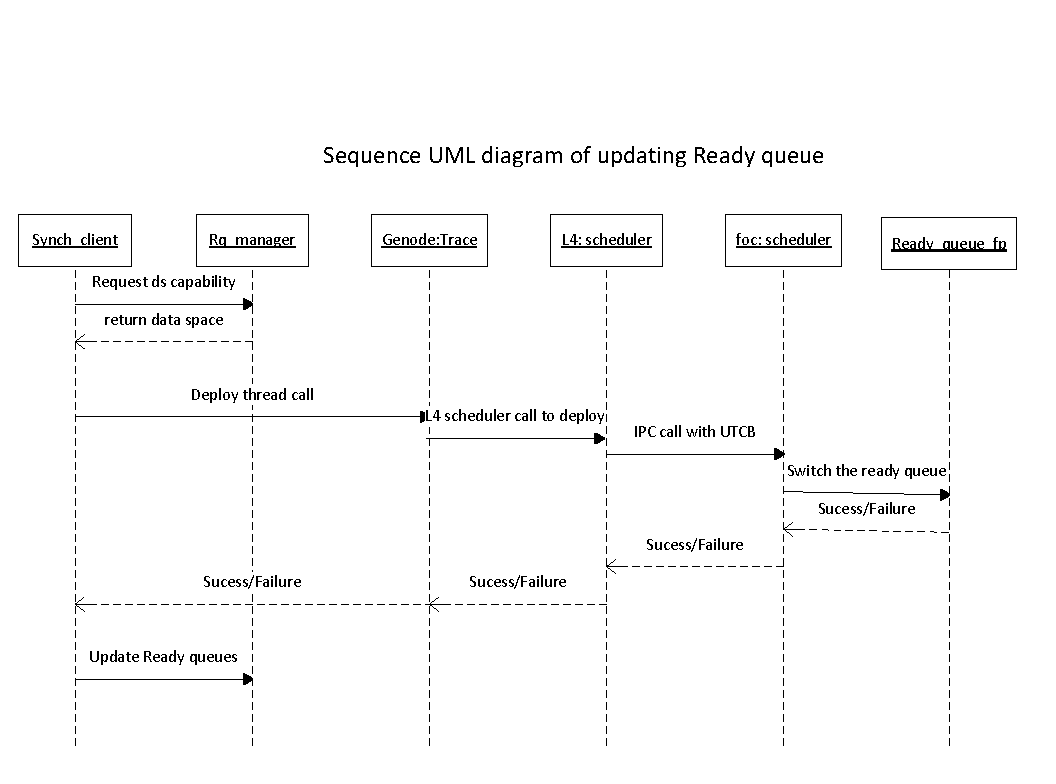
\includegraphics[width=1.0\linewidth]{figures/sequence_classUpdate}
\caption{Sequence diagram of updating ready queue from the Genode component}
\label{fig:sequence_classUpdate}
\end{figure}

%TODO explain the sequence diaram here
%TODO Add articles
%TODo remove commas from figure

\section{Rq\_manager module}

 The class \texttt{Rq\_manager} is the driver class of this component. It creates and maintains multiple ready queues at the user-level component, where each queue is of type Rq\_buffer. The Rq\_buffer is a template class, which implements a circular array by using the Genode dataspace. Each entry in the Genode dataspace is a circular array of type Rq\_task struct, which represents a Genode thread.

The code listing \ref{rqmanager} shows the implementation of \texttt{Rq\_manager} class. The constructor of \texttt{Rq\_manager} class first gets the number of available cores from Monitoring agent, then the \texttt{\_init\_rq()} function initializes the ready queues by using \texttt{init\_w\_shared\_ds} method from the Rq\_buffer class. The \texttt{Rq\_manager} provides enqueue and dequeue operations for the manipulation of ready queue.

\begin{lstlisting}[caption={Rq\_manager class},label={rqmanager}, style=customcpp]
class Rq_manager
{	

		private:

			int _num_cores = 0;
			Rq_buffer<Rq_task> *_rqs; /* array of ring buffers (Rq_buffer with fixed size) */
			
			int _set_ncores(int);

		public:

			int enq(int, Rq_task);
			int deq(int, Rq_task**);
			int get_num_rqs();
			Genode::Dataspace_capability get_core_rq_ds(int);

			Rq_manager()
			{
				PINF("Value of available system cores not provided -> set to 2.");

				_set_ncores(2);
				_init_rqs(100);
			}

			_init_rqs(int rq_size)
			{

				_rqs = new Rq_buffer<Rq_task>[_num_cores];

				for (int i = 0; i < _num_cores; i++) {
					_rqs[i].init_w_shared_ds(rq_size);
				}
				Genode::printf("New Rq_buffer created. Starting address is: %p.\n", _rqs);

				return 0;

			}
}
\end{lstlisting}

The Rq\_buffer is a template class, which represents the ready queue in the application side. It implements a circular array with fixed size. It uses \texttt{head} pointer, which points to the beginning of the array and \texttt{tail} pointer, which points to the end of the array. The elements are always inserted at tail pointer and removed from head. The pointers are wrapped around, whenever they reach the end of the array. The free space available between head and tail is represented by using a pointer called \texttt{window}. 

Rq\_buffer has enqueue and dequeue functionalities which can be called from \texttt{Rq\_manager} to insert or remove an element from ready queue. It also provides a functionality to initialize and create a shared dataspace. The code listing \ref{rqbuffer} shows, memory allocation for the shared dataspace and attaching it to the RM session of the component.

\begin{lstlisting}[caption={Allocating dataspace},label={rqbuffer}, style=customcpp]

	Genode::Dataspace_capability _ds; /* dataspace capability of the shared object */
	char *_ds_begin = nullptr;        /* pointer to the beginning of the shared dataspace */

		/* 
		 * create dataspace capability, i.e. mem is allocated,
		 * and attach the dataspace (the first address of the
		 * allocated mem) to _ds_begin. Then all the variables
		 * are set to the respective pointers in memory.
		 */
	_ds = Genode::env()->ram_session()->alloc(ds_size);
	_ds_begin = Genode::env()->rm_session()->attach(_ds);

\end{lstlisting}

The code listing \ref{rqtask} shows the Rq\_task structure which represents an entry in the ready queue buffer. It contains the parameters such as task\_id to identify a Genode task.

\begin{lstlisting}[caption={Rq\_task structure},label={rqtask}, style=customcpp]
 struct Rq_task
 	{
 
			unsigned long task_id;
 			int wcet;
 			bool valid;
 
 	};
\end{lstlisting}

The access to this shared dataspace must be synchronized since both the \texttt{Controller} and the \texttt{Synch\_client} use  it. This is done by locks provided from Genode.

\section{Synch\_client module}
The \texttt{Synch\_client} class represents a Genode component which controls the process of scheduler ready queue update. It acts as a client in Genode by using the services of the \texttt{Rq\_manager} and accesses the shared dataspace. The \texttt{Controller} and the \texttt{Synch\_client} interaction is that of a producer-consumer relationship. The producer (\texttt{Controller}) decides and produces(puts it in a buffer) a thread that needs to be executed and consumer(\texttt{Synch\_client}) picks the threads to the kernel ready queue.

%TODO insert flowchart
The initial communication with the \texttt{Rq\_manager} is governed by RPC call. In order to make an RPC call, it creates a Connection object. As explained before there are a number of pointers used for manipulating the circular buffer. The different pointers used are:

\begin{labeling}{pointers}
	\item [\_rqbufp] Hold the pointer to the Rq\_buffer type
	\item [\_lock] Lock needed to ensure mutual exclusion
	\item [\_head] Head pointer, points to the start of Rq\_buffer
	\item [\_tail] Tail pointer, points to end of Rq\_buffer
	\item [\_window] The window of free spaces available in between head and tail
\end{labeling}
 
There can be more than one ready queue. So, we need multiple pointers of each type. The data type \texttt{vector} is used to represent the pointers as the available number of ready queues is unknown at the creation time. The declaration of all the data structures can be seen in the listing \ref{synchdata}. 

\begin{lstlisting}[caption={Data structures used in Synch\_client},label={synchdata}, style=customcpp]
	Rq_manager::Connection rqm;
	
	/* using vectors since we dont know the size initially */
	std::vector<int *> _rqbufp;
	std::vector<int *> _lock;
	std::vector<int *> head; 
	std::vector<int *> tail; 
	std::vector<int *> window;
	
	std::vector<Dataspace_capability> dsc;
	std::vector<Rq_manager::Rq_task*> buf;
\end{lstlisting}

We can use the Connection object created to make RPC calls to the\texttt{Rq\_manager}. The first RPC call is to obtain the number of ready queues available. For each ready queue available, it has to make an RPC call to get the dataspace capability and attach to the local RM session and initialize all the pointers shown in the listing \ref{synchdata}. 

After everything has been initialized the \texttt{Synch\_client} runs in an infinite loop. For each ready queue it tries to obtain the lock, if the locking is successful then it schedules the threads available in the ready queue. The infinite loop has two goals. First, it has to ensure that it moves on to the next ready queue so that the threads in other queues also gets scheduled. Second, is to reduce the amount of time spent in the critical section as little as possible. In order to achieve the above mentioned goals, the ids of the threads/tasks are copied to a local buffer, head and tail pointers updated and the lock is released. By this way the scheduling of threads by calling of Genode API is kept outside the critical section.

One more option to reduce the critical section is to have separate threads working on each of the ready queues. Each thread will be working on a different ready queue and there is no shared data between these thread, which guarantees the second goal mentioned for the infinite loop. 
 
\section{Ready queue update Mechanism}

The ready queue update mechanism follows the series of calls which are shown in sequence diagram \ref{fig:sequence_classUpdate}. The following subsections explain the implementation of the modules described in \ref{design:rqupdate}.

\subsection{Genode code changes}

Genode should provide a way to the application for calling the L4 API calls. In the present Genode code the L4 APIs calls for scheduling threads are done from \texttt{Platform\_thread.cpp}, where the thread gets created. But the \texttt{Platform\_thread} is not accessible from the application, as it doesn't provide any RPC interface for applications to make use of its services. The only way that the components communicate in Genode is by using RPC calls. So an RPC call needs to be provided for the components to use it. As of now this call is kept in \texttt{Trace} service. The trace service is being used by the monitoring agent already to obtain the data from the Genode. The Trace service has been extended to provide an API, which can be used to from the \texttt{Synch\_client} component.

The \texttt{base/src/trace/trace\_session\_component.cc} contain the API definition, in which it takes a structure argument of threads and calls the L4 scheduler call.

\subsection{L4 API calls} \label{imp:l4api}
I introduced a new L4 API which can be called from the Genode. The APi takes the following arguments:

\begin{itemize}
\item l4\_cap\_idx\_t: It takes a kernel object which is scheduler object.  

\item l4\_sched\_thread\_list: This is a structure which can be seen in \ref{l4api}, which has an array to hold the list of threads and the priorities for the same threads. 

\end{itemize}

The code listing  \ref{l4api} shows the l4\_sched\_thread\_list structure and the L4 API call which is called from Genode and this code is in \texttt{foc/l4/l4sys/scheduler.h}.
\begin{lstlisting}[caption={L4 scheduler API in scheduler.h},label={l4api}, style=customcpp]

typedef struct l4_sched_thread_list
{
	l4_cap_idx_t list[10];
	unsigned prio[10];
	int n;
}l4_sched_thread_list;

L4_INLINE l4_msgtag_t
l4_scheduler_deploy_thread(l4_cap_idx_t scheduler,
		l4_sched_thread_list thread) L4_NOTHROW
{
  return l4_scheduler_deploy_thread_u(scheduler, thread, l4_utcb());
}
\end{lstlisting}

The deploy thread function call has to fill the UTCB message registers and make an IPC call to the scheduler kernel object. The first register(mr[0]) is populated with the type of operation that the scheduler should do to with the information, in this case it is L4\_SCHEDULER\_DEPLOY\_THREAD\_OP. The second register is populated using a call to l4\_map\_obj\_control function, which returns a word. This word identifies the kernel objects, which come after this word in the message registers. After the map object control word, thread objects are filled in the message registers in the form of L4 flex pages. An L4 flex page represents a naturally aligned area of mappable space, such as memory, I/O-ports, and capabilities (kernel objects), in this case L4 flex represents thread object.
For each thread id which is sent an L4 flex page is created and stored in the UTCB message registers. The L4 API makes an IPC call to the kernel scheduler object. 

The code listing \ref{l4apimp} shows the L4 scheduler API implementation.

\begin{lstlisting}[caption={L4 scheduler API implementation},label={l4apimp}, style=customcpp]
L4_INLINE l4_msgtag_t
l4_scheduler_deploy_thread_u(l4_cap_idx_t scheduler, l4_sched_thread_list thread,
			  l4_utcb_t *utcb) L4_NOTHROW
{
  l4_msg_regs_t *m = l4_utcb_mr_u(utcb);
  m->mr[0] = L4_SCHEDULER_DEPLOY_THREAD_OP;
  m->mr[1] = l4_map_obj_control(0, 0);

  for(int i = 0; i < thread.n; i++){
	  m->mr[i+1] = l4_obj_fpage(thread.list[i], 0, L4_FPAGE_RWX).raw;
  }
  
  return l4_ipc_call(scheduler, utcb, l4_msgtag(L4_PROTO_SCHEDULER, thread.n+1, 1, 0), L4_IPC_NEVER);
  }
\end{lstlisting}
  
\section{Fiasco.OC code changes}
Fiasco.OC code changes are made in several files to incorporate the ready queue update mechanism in the kernel and following sections explain the code changes in each file.

\subsection{Scheduler.cpp}

The \texttt{l4\_ipc\_call} from the scheduler.h invokes \texttt{kinvoke} function. The first parameter of the UTCB is decoded to find out the operation that is involved in. The operation in this case was set to \texttt{deploy\_thread} and which calls the function \texttt{sys\_deploy\_thread}, which can be seen in code listing \ref{sysdeploycode}. It runs a for loop to get the number of available threads. The associated flex page is derived from the sent items and a look up is performed to obtain the thread objects. The thread objects can be used to obtain the scheduler context which they are associated with. The scheduler context objects are used to create ready queue list(Fp\_list). This list is used to switch the actual ready queue of the scheduler.

The specified ready queue of the CPU can be obtained if the CPU was specified from the \texttt{Controller} otherwise the ready queue of the threads home CPU can be used. The current implementation creates and works with fixed priority list, however, this can be extended easily to create the corresponding ready queue list. If there is only one thread the \texttt{ready\_enqueue} function can be called instead of exchanging the complete list.


\begin{lstlisting}[caption={Thread extraction and ready list creation},label=sysdeploycode, style=customcpp]
Scheduler::sys_deploy_thread(L4_fpage::Rights, Syscall_frame *f, Utcb const *utcb)
{
	printf("[Scheduler: sys_deploy_thread] 1\n");
	L4_msg_tag const tag = f->tag();
	Cpu_number const curr_cpu = current_cpu();

	Obj_space *s = current()->space();
	assert(s);

	typedef Sched_context::Fp_list List;

	List list;
	
	for(int i = 6 ; i <= tag.words(); i++){
				
				/*
				 *	Get the messages in an iterator
				 */
				L4_snd_item_iter snd_items(utcb, i);

				/*
				 * Check if the items exist
				 */
				if (EXPECT_FALSE(!tag.items() || !snd_items.next()))
					return commit_result(-L4_err::EInval);

				L4_fpage _thread(snd_items.get()->d);

				if (EXPECT_FALSE(!_thread.is_objpage()))
					return commit_result(-L4_err::EInval);

				/*
				 * Do a look up to get the corresponding thread and cast 
				 * it to Thread_object type
				 */
				Thread *thread = Kobject::dcast<Thread_object*>(s->lookup_local(_thread.obj_index()));
				if (!thread)
					return commit_result(-L4_err::EInval);

				printf("[Scheduler:sys_deploy] Thread to be scheduled: %lx\n", thread->dbg_id());

				list.push(thread->sched_context(), List::Front);

				Sched_context::Ready_queue &rq = Sched_context::rq.cpu(thread->home_cpu());

				if(i==tag.words()){
				 rq.switch_ready_queue(&list, 100);
				}
		}
}
\end{lstlisting}

\subsection{sched\_context-fp\_EDF.cpp}

This class implements the major functionalities to handle the ready queues. This class contains the lists of both FP ready queue and EDF ready queue and serves as a wrapper class to both type of lists. Any call made to access the either of the ready queue, goes through this class. The decision to call the specific ready queue function is made according to the type of the scheduler in use.

Since this work was involved with fixed priority lists, the check to find out the type of scheduler in use is not made and default is to use the FP ready queue. However, it can be extended easily to work with both the lists. Code listing \ref{switchrq} shows the calling of the function to fixed priority ready queue.

\begin{lstlisting}[caption={Exchanging the ready queue},label=switchrq, style=customcpp]
IMPLEMENT
bool
Sched_context::Ready_queue_base::switch_rq(Fp_list *list, unsigned prio)
{
	return fp_rq.switch_rq(list, prio);
}
\end{lstlisting}

\section{Synchronization method}\label{imp:sync}

The ready queue contains the scheduler contexts which belongs to the threads and which can run next. Modifying the ready queue list is a critical section and mutual exclusive access must be guaranteed. In a uniprocessor implementation this can work with the CPU lock, which disables the interrupts on the local CPU and no other threads will get CPU time in the middle of ready queue manipulation. For SMP systems the kernel must use a ready list local to the CPU and advantages of using the per CPU data is explained in the section \ref{foundations}. Fiasco.OC implements a per CPU variable which is used towards synchronization. When using per CPU variable the exclusive access to this variable is guaranteed by disabling the CPU preemption and once the access is finished the CPU preemption is enabled. By this way, if any CPU is in the middle of critical section, no thread is allowed to replace the current operation. 

The present method uses the per CPU variable method where it locks the CPU before exchanging the CPU list. The software transaction memory method was implemented but testing that method was a problem since using of SMT forces the GCC compiler required pthreads library to be present which was not possible to include to Fiasco.OC. The SMT method would eliminate the necessary to preempt the CPU since it executes all the exchange the instructions in one transaction.

A check is made in scheduler.cpp to find out if the ready queue is empty. If the ready queue is empty or it contains the idle thread then the immediate call is made to exchange the list. The static point in time method is to check if a thread from this ready list getting executed, if the thread is running
the exchange call waits till the scheduler takes the control back and thread list is exchanged. This is checked in the call from \texttt{schedule\_in\_progress} flag. 


\subsection{Ready\_queue\_fp.cpp}
Hereinafter the list that is sent is referred as new list and the list to be exchanged is referred as old list. Once the fixed priority ready queue is decided to be exchanged the new list and the priority is sent to the \texttt{switch\_rq} function from sched\_context-fp\_EDF class. It is assumed at this point that the new list contains the threads that are necessary to execute the threads, which include the idle thread, pager threads. The Fiasco.OC uses an idle thread which keeps the CPU busy when there are no threads are to be executed. The idle thread needs to be kept in the new list if it's not existing already. The old list can be used to identify the idle thread, which sits in the end of the old list. The pager thread is nece

The exchange of the list is a simple operation of changing the head pointers. The cyclic list is implemented in a file called \texttt{dlist}. I implemented a a function \texttt{exchange} which takes the list to be exchanged with the present list and sets the head of the old list to the new list. 

The listing \ref{rq_exchange} shows the \texttt{switch\_rq} function.

 \begin{lstlisting}[caption={Exchanging the ready queue},label=rq_exchange, style=customcpp]
 bool switch_rq(List *list, unsigned prio) {
   		assert_kdb(cpu_lock.test());
 
   		prio_next[prio].exchange(list);
 
   		//prio_next[prio].rotate_to(*++List::iter(list->front()));
 
   		typename List::BaseIterator it = List::iter(prio_next[prio].front());
   		dbgprintf("After exchange fp_rq: ");
   		do
   		{
   			dbgprintf("%lx => ",Kobject_dbg::obj_to_id(it->context()));
   		}while (++it != List::iter(prio_next[prio].front()));
   		dbgprintf("end\n");
 
   		return true;
   	}
 
\end{lstlisting} 

\section{Creating a new kernel object in Fiasco.OC}\label{implement:kernelobject}
In this section creating a new kernel object is explained, that can be utilized to make a dedicated work in the kernel. The following changes are required to create kernel object and compile it. A new class should be created, which inherits \texttt{Icu\_h<object name>} and
\texttt{Irq\_chip\_soft} classes. The class has to declare this as kernel object using a macro (FIASCO\_DECLARE\_KOBJ()) provided from Fiasco.OC and the memory is allocated outside the class by defining the kernel object and sending the class name as a parameter. The class has to have a static object created inside the class and an interrupt request(Irq\_base) object defined in it. In the constructor of the class it is important to register this object to initial kernel objects. 

The class definition and the registering of kernel object can be seen in listing \ref{kobject}. The new object is called \texttt{RQ\_manager}, which should take care of the ready queue handling.

\begin{lstlisting}[caption={Creating new kernel object},label=kobject, style=customcpp]
class RQ_manager : public Icu_h<RQ_manager>, public Irq_chip_soft
{
  FIASCO_DECLARE_KOBJ();
  typedef Icu_h<RQ_manager> Icu;

public:
  enum Operation
  {
	RQ_info = 0,
	Schedule_thread = 1,
  };

  static RQ_manager rq_manager;
private:
  Irq_base *_irq;
};

FIASCO_DEFINE_KOBJ(RQ_manager);

PUBLIC inline
RQ_manager::RQ_manager() : _irq(0)
{
  initial_kobjects.register_obj(this, 8);
}

PUBLIC
L4_msg_tag
RQ_manager::kinvoke(L4_obj_ref ref, L4_fpage::Rights rights, Syscall_frame *f,
                   Utcb const *iutcb, Utcb *outcb)
{
}

enum Protocol{
  Label_rq_manager = -22L,   // Protocol ID for rq manager objects<l4_types.cpp>
}
enum l4_msgtag_protocol{
L4_PROTO_RQ_MANAGER = -22L, //Protocol for messages to a rq_manager object<types.h>
}

static Cap_index const C_rq_manager = Cap_index(8); //kernel-thread-std.cpp
\end{lstlisting}

This class should implement few of the functions from the inherited classes such as \texttt{icu\_bind\_irq} and \texttt{icu\_set\_mode} and a \texttt{kinvoke} call which the Fiasco uses it to do interprocess communication.

This created kernel object needs to be associate with protocol ID. These protocol IDs are used for either
kernel implemented objects and this is assigned in the \texttt{l4\_types.h}, protocol section of the
l4\_msg\_tag and also it needs to be assigned with l4\_msgtag\_protocol. This kernel object is assigned a \texttt{Cap\_index} which it was registered against.
\chapter{Testing and Results}\label{chap:testing}
In this chapter testing of the modules is explained. The complete Observer-Controller architecture is still in development stage, so the integration testing of the complete architecture described previously was not possible. So the user-level Synchronization module(Synchronization 1) is tested separately from the kernel Synchronization module (Synchronization 2). The user-level component is tested to make sure the dataspace  access is possible and it can communicate with the \texttt{Controller} via the dataspace.

To test the kernel ready queue update mechanism as a standalone component, the Genode thread ids need to be sent from a user-level component. Therefore, a new Genode component called \texttt{gehello} was developed as a utility to test the kernel module. It creates a set of threads and passes them to the kernel. In order to obtain the thread ids required Genode's trace facility is extended to get the thread ids from platform thread class of Genode OS framework which is explained in the next section.

\section{Test Utility Using Trace: gehello}

\begin{figure}[h]
\centering
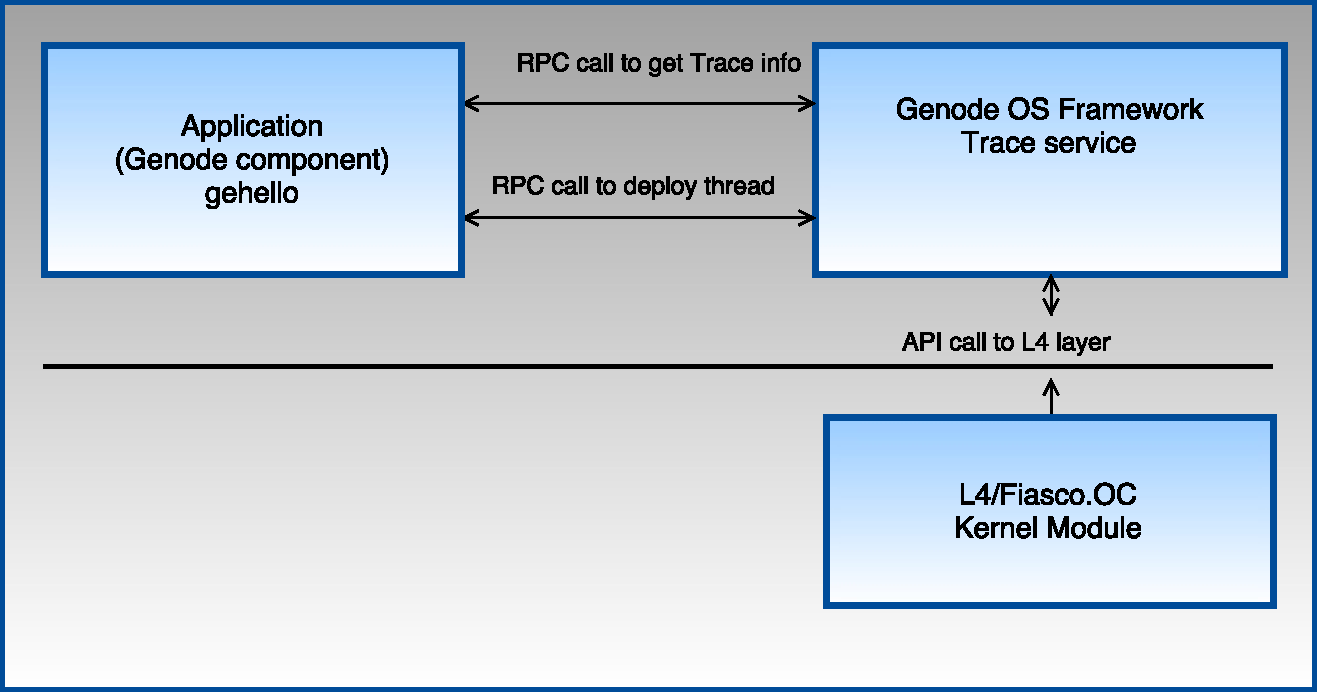
\includegraphics[width=0.7\linewidth]{figures/test1}
\caption{Test utility design using Trace service}
\label{fig:test}
\end{figure}

The gehello test utility is implemented as a Genode component, it creates a set of threads and passes them to the kernel module to update them to the ready queue. In order to create the threads, it has to inherit the Genode's thread class and specify the stack size as a template parameter. 

The Listing \ref{gehello} shows this thread creation. The class \texttt{Mythread} inherits the Genode's Thread class. It has a constructor, which in turn calls the base class's constructor with a string (name of the thread) as a parameter. This call goes to platform thread class to create the thread as explained in section \ref{foundations:thread_creation}. The entry function of this thread just does a print on the  command line. The \texttt{Thread\_creator} class creates the \texttt{Mythread} class object(myt). It has a run\_thread function which calls the start method associated with the thread. The start method invokes the entry function defined in the \texttt{Mythread} class and it has to call join method of the thread to end specify the end of thread's execution.

\begin{lstlisting}[caption={gehello trace utility},label={gehello}, style=customcpp]
class Mythread : public Genode::Thread<2*4096>
{
	public:
		Mythread() : Thread("MyThread") { }
		void entry(){
			printf("I'm a thread\n");
			// Some useful work
		}
};
class Thread_creator
{
	Mythread myt;
	public:
		int run_thread(){
				myt.start();
				Genode::Thread_capability mycap = myt.cap();
				PINF("Got Thread capability information. %lx\n", myt.tid());
				myt.join();
		}
};
\end{lstlisting}

\subsection{Trace Extension}
The information about the Genode's tasks/thread can be obtained from using Core's Trace service. Trace service was extended to get the thread information from Genode's platform thread class. 

The \texttt{source\_registry.h} has a information struct called \texttt{Info}, which is returned by Trace service to an application. A new element has been added to the Info struct for thread id. 


\begin{lstlisting}[style=customcpp]
	struct Info
		{
			Session_label      label;
			Thread_name        name;
			Execution_time     execution_time;
			Affinity::Location affinity;
			unsigned 		   prio;
			unsigned long	   thread_id;
		};
\end{lstlisting}


The \texttt{info()} method of the \texttt{subject\_registry} calls the {trace\_source\_info()} function of the \texttt{Cpu\_session\_component} class to obtain the thread information. The class \texttt{Cpu\_session\_component} has the \texttt{platform thread} object and returns the thread id.

\begin{lstlisting}[style=customcpp]
	Trace::Source::Info trace_source_info() const
			{
				return { _session_label, _name,
				         _platform_thread.execution_time(),
				         _platform_thread.affinity(),
						 _platform_thread.prio(),
						 _platform_thread.thread_id()};
			}
\end{lstlisting}


Platform thread class is extended with a method to return the thread's local id as shown below.

\begin{lstlisting}[style=customcpp]
unsigned long Platform_thread::thread_id() const
{
	return _thread.local.dst();
}
\end{lstlisting}

\section{Building the System}
The Synchronization module is tested on Ubuntu 14.04 LTS using QEMU to virtualize the hardware (PBX-A9) board. The following subsections explain the installing dependencies and compiling Genode along with the Fiasco.OC.

The changed Fiasco.OC and Genode source can be downloaded from \cite{git_synccode}.

\subsection{Installing Dependencies}

Genode and Fiasco.OC require these following packages to be installed.

\begin{itemize}

\item GNU Make version 3.81 or newer

\item libSDL-dev

\item tclsh and expect

\item byacc

\item QEMU: Required fir virtualizing the hardware.
\end{itemize}

Another option is to install the pre-compiled Genode tool chain for Linux available in Genode \href{http://genode.org/download/tool-chain}{website}.

\subsection{Compiling the gehello Application}
After installing the dependencies, clone the Genode operating system branch \texttt{focnados} from GitHub \href{https://github.com/702nADOS/genode-Synchronization}{repository}.

Once the Genode is downloaded prepare the Fiasco.OC kernel by issuing \textit{make-prepare} command in \textit{repos/base-focnados} folder.  But this would use the default Fiasco.OC code. In order to use the modified code for the thesis the \textit{port/focnados.port} file should be updated to access the code from the above mentioned GitHub repository.

Create a build directory using Genode tool for pbxa9 board using the below command
\begin{verbatim}
$ ./tool/create_builddir focnados_pbxa9
\end{verbatim}

The \texttt{gehello} application exists in the repos folder. By issuing the below make command in the build directory, the \texttt{gehello}  application can be built and tested. The expected output is given in the section \ref{testing:results}.

\begin{verbatim}
$ make -j4 run/gehello
\end{verbatim}

\section{Results}\label{testing:results}
The \texttt{gehello} application creates five threads and the Trace service returns the thread information to the user-space application. Listing \ref{gehellotrace} shows the information returned from the Trace. The names are compared to find out the threads created by the \texttt{gehello} application and these thread ids are selected and sent to the kernel using the Genode API. 

\begin{lstlisting}[caption={The returned information from the Trace service},label={gehellotrace}, style=customcpp]
ID:11 0 prio:128  thread_id: 293000 init 
ID:9 0 prio:128  thread_id: 2c0000 init -> gehello name:gehello
ID:8 0 prio:128  thread_id: 2e1000 init -> gehello name:MyThread
ID:7 0 prio:128  thread_id: 2e6000 init -> timer name:timer_drv_ep
ID:6 0 prio:128  thread_id: 2ec000 init -> gehello name:MyThread
ID:5 0 prio:128  thread_id: 2f6000 init -> gehello name:MyThread
ID:4 0 prio:128  thread_id: 2fd000 init -> timer name:timeout_scheduler
ID:3 0 prio:128  thread_id: 301000 init -> gehello name:MyThread
ID:2 0 prio:128  thread_id: 30b000 init -> gehello name:MyThread
ID:1 0 prio:128  thread_id: 317000 init -> timer name:signal handler
ID:0 0 prio:128  thread_id: 32c000 init -> gehello name:signal handler
\end{lstlisting}

The kernel threads are then identified in the kernel and added to the run queue. Listing \ref{kernelthreads} shows the kernel thread ids and the updated ready queue, when updating single thread at a time and  the updated threads start execution when the \texttt{gehello} application starts the threads.

\begin{lstlisting}[caption={The kernel thread ids and ready queue update},label={kernelthreads}, style=customcpp]

[Scheduler:sys_deploy] Thread to be scheduled: cd
fp_rq: cd => d => e9 => end

[Scheduler:sys_deploy] Thread to be scheduled: d8
fp_rq: d8 => cd => d => e9 => end

[Scheduler:sys_deploy] Thread to be scheduled: e2
fp_rq: e2 => d8 => cd => d => e9 => end

The thread execution:
[Platform_thread: start] 2e1000 started!
[init -> gehello] Got Thread capability information. c000

[init -> gehello] I am a thread!

[Platform_thread: start] 2ec000 started!
[init -> gehello] Got Thread capability information. f000

[init -> gehello] I am a thread!
\end{lstlisting}


\chapter{Summary, Future Work and Conclusion}
This chapter summarizes the thesis, discusses the importance of the work and findings, outlines the limitations and indicates directions for future work. 

This chapter has been divided into four sections. Section \ref{summary} is a summary of the thesis. Thesis contributions and limitations are discussed in \ref{disc}. Section \ref{futurework} outlines the possible future work, and Section \ref{con} concludes the thesis.

\section{Summary of the Thesis} \label{summary}
This thesis introduced a method for updating the task ready queues in Genode and L4/Fiasco.OC system and the motivation for developing the Synchronization module. The Synchronization module is used in the Observer-Controller architecture.

Chapter 2 gave an overview of the related work. The work done by H{\"a}cker in his bachelor thesis served as a basis for current thesis work. There are lock-based and lock-free synchronization methods available and each type has certain benefits associated with them in terms of \textit{implementation, read and write speed, security, deadlocks}. The lock-free methods, Read-Copy Update(RCU) and Software Transactional Memory (STM) are better suited for this thesis work.

Chapter 3 discussed the concepts necessary to understand the thesis. Genode OS framework is a tool kit for building special purpose operating system which can be used to build safe, secure and robust operating systems. It has a recursive tree structure and each node of the tree is owned by its parent, which has access to its own sandbox. It can be used with different microkernels. L4/Fiasco.OC is the preferred choice of microkernel for KIA4Sm project, since it offers many features such as, paravirtualization, multi processor support etc. This is a object capability system, where everything in kernel is represented as an object and they interact with each other through a kernel provided IPC mechanism. The thread execution in kernel is divided between execution context, which takes care of execution parameters and scheduling context object, which holds scheduling parameters.

Chapter 4 and 5 explained the design and implementation details of the thesis. The communication between the Controller and Synchronization module is that of a producer-consumer relationship and the communication between these two modules is handled by shared dataspace, which is synchronized by using the locks provided from Genode. The limitations in accessing the ready queue from the user-level application, led to the development of kernel module. The application interacts with the Genode API, which intern calls the L4 layer. The L4 layer makes the flex pages for the threads being sent from Genode and send them to the scheduler kernel object with an IPC call. The scheduler decides the right time for updating ready queue and updates the threads. A new ready queue list can be created with the threads and exchange with the actual ready queue or existing ready queue can be updated.

In Chapter 6, the testing of the individual components is described. Since the integration testing was not possible the individual components are tested. The trace service of Genode is extended to return the Genode thread ids, which are sent to the kernel module to update them to the ready queue.

\section{Discussion} \label{disc}
\subsection{Thesis Contribution}
This thesis has developed a method for updating the kernel ready queue. A user-level component has been developed to handle the communication with the Controller. The developed kernel module handles the ready queue update mechanism. The thesis gives insights to the working environment of Fiasco.OC kernel and its interaction with Genode OS framework. The thread creation model in Genode and the thread migration in L4/Fiasco.OC is explained in details to understand the scheduling method of the L4/Fiasco.OC scheduler.

\subsection{Limitations}
The presented design in this thesis is a decent method to update the task ready queue of the scheduler. However, there exists a few limitations to the method presented. First the user-level application handles each ready queue one at a time and has to wait till it acquires the lock. This may lead to starvation of threads. The user-level Genode component cannot access the kernel ready queue list  directly and also it cannot make calls to L4 API layer of the kernel. This limits the scope of the user-level component. The thread update to the ready queue works well and the execution of the thread continues and creating a new ready queue list to exchange with the actual ready queue happens, however, the ready queue exchange mechanism doesn't ensure the thread execution. The current implementation of kernel module is limited to work with fixed priority scheduler.

\section{Future Work}\label{futurework}
This section describes the ideas for future research to be done on this concept. Further investigations should be done to identify the best approach to integrate the Controller and the Synchronization module. The proposed idea for integration is, the Observer gathers data including the Genode thread ids to the Controller and the Controller has to take decisions on scheduling and make the corresponding thread ids available in the shared dataspace. The user-level Synchronization module can read this dataspace and update them to ready queue using kernel module. And also the kernel module extension is required to make it work with the different types of schedulers.

The initial aim of the thesis was to develop a high-level component for ready queue update. However, this had to be changed since the ready queue was not accessible from a high-level component. Further work should be carried out find out if a user-level component can replace the kernel module's work. The communication between user-level module to kernel module involves many API calls, further research to be done on this regard to reduce the number of API calls.

\section{Conclusion}\label{con}
The Synchronization module developed in this thesis is a decent method for updating the threads to kernel ready queue. It serves as a good starting point for the \texttt{Observer-Controller} architecture's goal of having a user-level component for ready queue update. However, this module can be extended to suite the overall goal of the KIA4SM project.
% TODO: add more chapters here

\appendix{}

\microtypesetup{protrusion=false}
\listoffigures{}
\afterpage{\blankpage}
\listoftables{}
\afterpage{\blankpage}
\microtypesetup{protrusion=true}


\printbibliography{}

\end{document}
